\documentclass[10pt,a4paper]{ctexart}
\usepackage[latin1]{inputenc}
\usepackage{amsmath}
\usepackage{amsfonts}
\usepackage{amssymb}
\usepackage{graphicx}
\author{吴秉哲}
\title{Extracted the style from the image\\with Deep Neural Network}
\begin{document}
	\maketitle
	\begin{abstract}
		在视觉艺术的领域,尤其是在绘画方面,画家已经能通过自己的经验和技术进行创作出一副独特的复杂的艺术作品,这些作品的内容和
        风格的联系十分复杂。在计算机视觉领域,由于卷积神经网络的兴起,一些传统的任务比如物体定位和物体识别已经取得了很大的进步。尤其是
        是物体识别已经有算法在大规模图片识别(imageNet 图片数据集)的任务上达到了类人的表现\cite{Krizhevsky2012ImageNet},其他方面,由于GPU
        通用计算\cite{Deng2012Large}的发展,人们已经有能力进行深度人工神经网络的训练(2014年ImageNet挑战赛的冠军使用的网络模型已经到了19层)。
        在这次的期末项目中,我会使用深层的卷积神经网络来提取一副图像的物体和另一副绘画的艺术风格,并将它们结合在一起,形成一副
        全新的图片。项目中使用的算法也提供一个途径帮助计算机理解人类是如何完成复杂的艺术创作的。
	\end{abstract}
	\section{Introduction}
	在这次的项目中,我们主要使用一种特殊的人工神经网络,卷积神经网络。卷积神经网络可以理解为一个特征提取的网络,区别与传统的
    计算机视觉的方法,卷积神经网络会自动完成对图片特征的提取,在训练一个多层的卷积神经网络的时候,随着层数的增加,图片中物体
    的轮廓会越来越清晰,但是一些图片的细节会损失。根据卷积神经网络这个特点,我们在提取一张图片的具体内容(就是图片里面的一些物体,比如建筑,动物等)的时候,我们只需要根据每一个卷积层得到的特征图(即上一层图片进过这层卷积得到的图片),对特征图进行重建,我们就可以提取图片中
    内容的信息。在这次的期末项目中,我们主要利用网络中深层所得到的特征图进行重建得到图片的内容的信息。
	
    另一方面,为了提取一幅绘画作品的风格特征,在项目中我们设计了一个基于原始图片纹理信息的特征空间。我们使用的这一个特征空间
    建立在卷积神经网络每一层的特征图上,它们由这些特征图之间的相关性组成,通过这种取特征图之间相关性的做法(详细见方法篇),我们可以获得原始绘画作品的风格特征而不是画中具体的物体信息和物体之间的布局信息。
    为了方便,在下文中,我们将这样构建的特征空间称为风格特征空间。

    这样,有了上面的风格特征空间,我们可以在风格特征空间上通过一些方法重建一幅图片,使得这幅图片可以与原始的绘画作品的风格匹配。
	
	在这次的期末项目中,我们可以通过上面的方法分别获得一张图片的内容以及一张绘画作品的艺术风格,将它们混合在一起得到一张全新的图片。在项目中我们设计了一个基于原始图片纹理信息的特征空间中,为了展示这个效果,我们会将自己拍摄的一些图片和一些著名画家的油画作品的风格融合,具体的
    效果见实验结果.

    上面提到的图像的合成i(即一张图片的内容结合绘画作品的风格)是通过这样的方法:初始化一张白噪声图片,然后定义误差函数,即给定一张图片,
    这张图片与原始图片的内容的误差,以及和原始绘画作品的风格误差函数,训练的时候通过梯度下降法,最小化所定义的误差函数,这样初始化的那张
    白噪声图片就可以通过迭代形成最后我们想要得到的两种图片的融合。
	
    当然一幅图像的风格和内容是不可能完全分离开的,比如名画呐喊中的风格和图中出现的那个个人。当我们进行上述的图片合成的时候,
    我们不会得到一张图片,它既完美匹配一张图片的内容,又和给定的绘画作品的风格匹配得很好。这里就存在一个平衡点,在项目中为了寻找
    这个平衡点,我们主要通过改变我们的误差函数中风格误差和内容误差的系数得到。

    在这次项目中,我们基于一台带GPU(Titan X)的实现了一个自动的智能系统,输入两张图片(一张是你想要的内容和另一张你想要的风格),得到
    一张融合两种图片的全新的图片。我们使用的神经网络模型是2014年获得ImageNet挑战赛冠军使用的模型VGGNET。
    
    这个报告的其余部分由下述的部分组成:第二个小节介绍关于卷积神经网络的基本理论和VGGNET这个模型的基本结构,在第二节中也会对我们
    使用的数据集(ImageNet DataSet)进行介绍。第三小节会对我们使用的图片生成方法进行严格的数学描述。第四小节会介绍我们实现这个智能系统
    的具体实现细节(包括网络的训练和合成图片的训练)。第四小节展示了最后实验的一些结果。
	\section{背景}
	\subsection{数据集合}
    ImageNet 图片数据库由 1500,0000 张标注图片组成,这些图片一共有22000个类别。这些图片通过亚马逊的标注系统人工标注。2010年,一项基于这个
    数据集合的大规模图像识别比赛(ILSVRC)开始举办,这个比赛选取ImageNet图片库的一个子集,这个子集有1000类图片,120000张训练图片我们项目中使用的
    神经网络模型就是基于这个图片库进行训练。

    这个数据库的图片有各种大小,所以在训练之前,我们对图片进行了预处理,基于线性插值的方法将每张训练图片下采样到 256*256.除了下采样,我们不对图片做任何其他的预处理。完成图片预处理之后,我们使用开源的深度学习框架Caffe\cite{jia2014caffe}训练我们的VGG 网络模型。
	\subsection{CNN Basics}
    卷积神经网络最早是受神经科学的启发而产生的(猫的大脑皮层的感受野是基于局部感知的)\cite{Hubel1962Receptive}。
    1998年Lecun提出了最早的卷积神经网络的结构LeNet用于手写字体的识别上,达到了商用标准。随着21世纪后GPU通用计算的发展,以及一些大型
    标注图片库的出现,CNN出现在了计算机视觉的领域内,在2012年的ImageNet 挑战赛上,多伦多大学的一个组使用了一个深层的卷积神经网络结构获得了第一名,与使用传统计算机视觉方法的第二名拉出了很大距离。
	自此卷积神经网络开始应用到一些传统的领域(比如模式识别,自然语言处理)。

    与传统的人工神经网络的结构相比,卷积神经网络采用权值共享和稀疏连接的策略大大减小了反向传播算法的计算量,也降低了模型的复杂度。
一个典型的卷积神经网络有两部分构成:一个特征提取器和一个分类器。特征提取器即为多层的卷积层,它将输入的图片通过卷积和
下采样等方式得到一系列原始图片的特征(保存在一系列特征图中),训练卷积神经网络就是完成计算机对图片的特征的提取,而不需要人工去
构造特征。这些提取的特征将会被送到分类器当中(通用的有SVM和多层感知器),达到对图片识别的效果。
	
一个卷积神经网络通常有多层结构。特征提取器就由多层卷积层和采样层构成,每一层的输入均为上一层通过卷积所得到的特征图。图一展示了一个典型
的卷积神经网络,卷积层接受 N 个特征图作为输入,每一个输入特征都与一个卷积核S做卷积,总共输出M(M对应与卷积核的个数)个特征图作为下层卷积层的输入。
	\begin{figure}[h]
		\centering
		{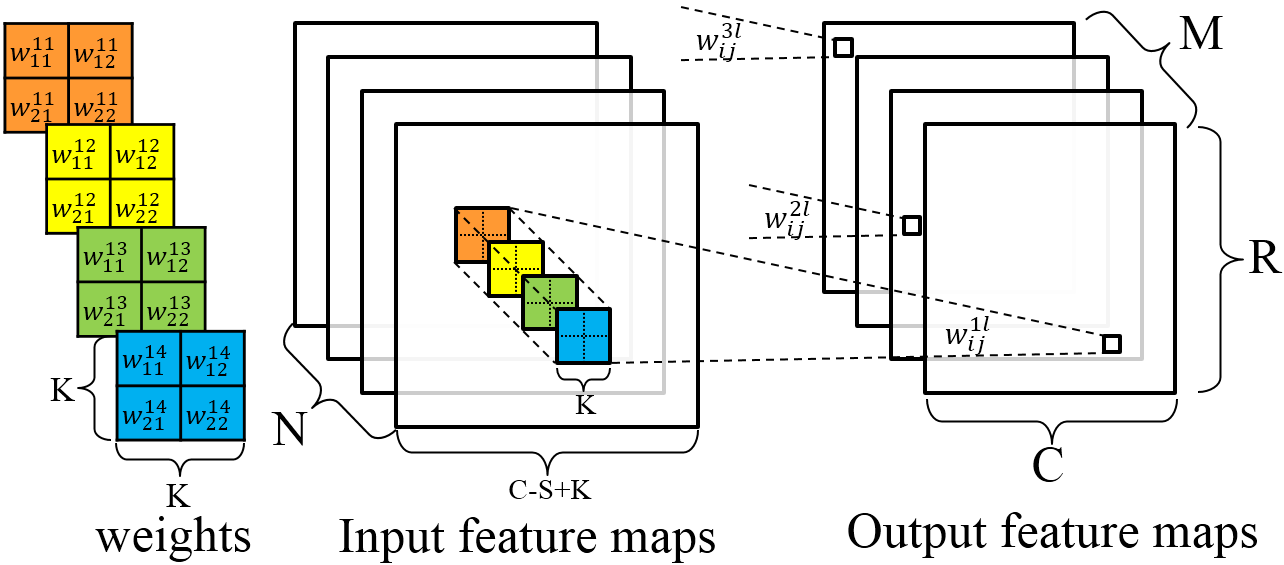
\includegraphics[width=0.8\linewidth]{convolve.png}}
		\caption{Graph of a convolutional layer}
		%	\label{fig_convolve}
	\end{figure}
	\subsection{VGG Model}
	\subsubsection{ARCHITECTURE}
    VGG 网络模型是一个卷积神经网络模型,他在一项图片识别的任务中达到了类人的表现,它的详细介绍可以参\cite{Simonyan2014Very}.
	
    在这次的期末项目中,我们使用\cite{Simonyan2014Very}中介绍的网络模型,将其应用于对我们数据集的训练。在训练的时候,输入图片的
    大小固定在225*225 ,图片为RGB格式,即有三个颜色通道。我们对图片进行如下的预处理:
    
    将图片通过线性插值的方法固定在网络输入所要求的大小,然后将图片每一个像素点的数值做归一化处理。
	
    不同于一些其他的卷积神经网络模型(比如AlexNet,LeNet),在VGG 的网络结构中,它的卷积核的维数很小,每一层卷积层的卷积核均为
    $3\times3$ (这已经是一个二维卷积所能达到的最小了,再小就是对图片的线性变化了)。在VGG的卷积层中,卷积核滑动的步长固定,在项目中
    我们取了符合二维卷积数学定义的1。模型的下采样层我选择了局部最大化采样,即在一个图像的局部选取局部像素值最大的一点代表这个局部
    的情况,这样可以达到对特征图降维的目的,下采样的范围定为2*2 ,即在特征图的每个2*2的像素块进行下采样。在\cite{Simonyan2014Very}描述的
    结构中,除了上述的卷积层和下采样层,之后还有三个全连接层(即传统的人工神经网络结构)进行对之前提取特征
    的分类,但是在我们的项目中,由于只需要将原始输入图片的特征提取出来即可,不需要分类,所以我们去掉了网络中的全连接层。
	
    所有隐含层使用的激活函数都是 ReLU,即 $ max(0,x)$。(也可以使用传统的比如sigmod函数,通过实验发现不同的激活函数差别不大)
	
    整个VGG 一共有16层卷积层,5个下采样层。
	整个网络的结构可以在宏观上展现为图二中的结构:
	\begin{figure}[h]
		\centering
		{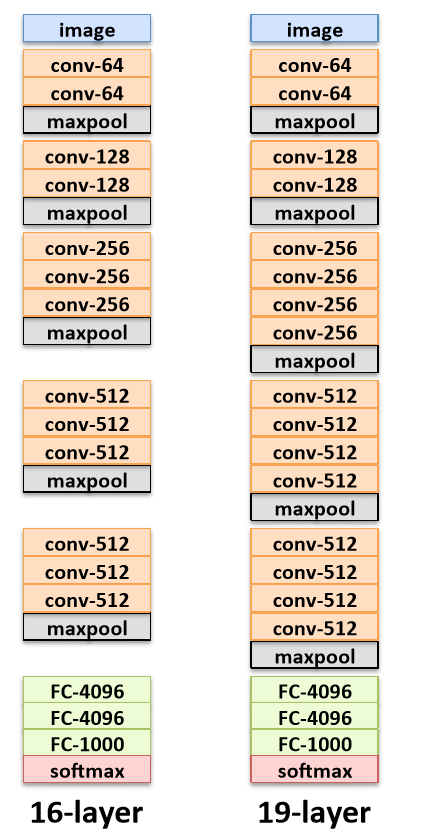
\includegraphics[width=0.8\linewidth]{vgg.png}}
		\caption{Graph of a convolutional layer}
		%	\label{fig_convolve}
	\end{figure}
	\section{方法}
    我们实验最后展现出来的结果是基于VGG的网络结构(见第二小节),在项目中我们会使用16个卷积层提供的特征来得到图片的内容
    和风格。我们不使用网络最后的全连接层。我们还会改变一些原来网络中下采样层的一些结构。下面分两个方向,即模型的训练和图片的
    合成两个方向来进行说明。
    \subsection{模型训练}
    我们在项目中使用深度学习的开源框架Caffe对数据集进行训练,针对大数据量的训练(我们最后训练使用的图片的存储大小为168个G),
    我们使用了GPU进行计算,在训练之前,也将所有的图片创建为一种高性能的存储格式(lmdb)。在这里列出我们训练的一些主要参数:
    初始学习率为0.01,初始动量为0.9,初始的权重分布选取为高斯分布,使用的优化算法为随机梯度下降法。最后训练完成的模型以
    google protobuffer的协议存储在二进制文件当中,之后通过lua中的loadcaffe模块调用模型文件。
    \subsection{合成图片}
    我们可以将卷积神经网络中的每一层的卷积核看为一个滤波器,图片与每个卷积核的卷积运算就可以当成是对
    图像的滤波下面引入一些记号。
    我们对网络其中一层卷积层(第l层卷积)引入记号即可,其他层类似。$N_l$ 个滤波器(即有$N_l$个卷积核,每个卷积核分别可以获得一种图像的特征),记这些卷
    积核展开为一维向量过后大小为 $M_l$,其中 $M_l$ 就是二维卷积核的高乘上宽
	
    这样 $l$层的经过滤波过后的图片可以存储在矩阵  $F^l \in R^{N_l\times M_l}$中 其中 $F_{ij}^{l}$是第
	 $i^{th}$ 个滤波器的响应函数.
     为了将图片的每一层特征图通过数值显式的表达出来,我们将对一个初始的白噪声图片通过梯度下降法迭代,从而寻找一副既能和一副照片的
     内容,也和一副绘画作品的风格匹配的图片出来。在这次的期末项目中
     我采取的算法是分别将这三张图片(即需要迭代的图片,原始的想要获得其内容的图片,原始的想要获得其
     风格的图片)传入之前训练好的神经网络模型中然后在神经网络的每一层我们会分别获得关于这些图片的一些特征图,
     我们在通过对他们特征图形成的特征空间进行误差的评估。
     
     下面分别讨论如何评价要迭代的图片和原始图片的内容的误差,与要迭代图片与原始绘画作品
     风格的误差。
     \subsubsection{内容误差}
	我们分别记 $\overrightarrow{p}$ 和$\overrightarrow{x}$ 是原始的我们想要获得其内容的照片和我们想要获取其内容的照片,记  $P^l$ 和 $F^l$ 分别是它们通过VGG网络第l层时的全体特征图,这样我们就可以定义两张图片在这一层的特征之间的均方误差函数,定义式如下:
	\begin{equation}
	L_{content} (\overrightarrow{p},\overrightarrow{x},l)= \frac{1}{2} \sum_{ij}
	(F_{ij}^{l}-P_{ij}^{l})^2
	\end{equation}
    有上面的表达式,我们可以得到误差函数(第l层,总体的误差函数会在本节最后定义)梯度的解析表达式:
	\begin{eqnarray}
	\dfrac{\partial L_{content}}{\partial F_{ij}^l}=\begin{cases}
	(F^l-P^l)_{ij} ,F_{ij}^l>0 \cr 0,otherwise
	\end{cases}
	\end{eqnarray}
	通过上面的梯度表达式,我们就可以根据误差的反向传播算法对要迭代的图片进行更新了。这样我们就可以先初始化一张随机图片(如这次项目
    中所用的白噪声图片),然后根据反向传播算法对其迭代,直到这张图片在这一层的经过卷积过后的特征图和我们想要获得图片类容的图片的特征图
    匹配即可。
	
    \subsubsection{风格误差}
    为了获得一幅图片的风格误差,我们首先需要定义一张图它的不同特征图之间的相关性,在这次项目中,我们采用如下的定义计算。
    On top of the CNN responses in each layer of the network we built a style representation that computes the correlatiddons between the different filter responses,where the expectation is taken over the spatial extend of the imput image.These feature correlations are given by the Gram
	matrix $G^l \in R^{N_l\times N_l}$,where $G_{ij}^l$ is the inner product between the vectorised feature map $i$ and $j$ in layer l:
	\begin{equation}
	G_{ij}^{l} = \sum_k F_{ik}^lF_{jk}^l	
	\end{equation}
	To generate a texture that matches the style of a given image,In the project,we use gradient descent from a white noise image to find another image that matches the style representation of the original image.This is
	done by minimising the mean-squared distance between the entries of the Gram matrix from the original image and the Gram matrix of the
	image to be generated .So let $\overrightarrow{a}$ and $\overrightarrow{x}$ be the original image and the image that is generated
	and $A^l$ and $G^l$ their respective style representations in layer l .The
	contribution of that layer to the total loss is then 
	\begin{equation}
	E_l = \dfrac{1}{4N_l^2M_l^2}\sum_{i,j}(G_{i,j}^l - A_{i,j}^l)^2
	\end{equation}
	and the total losss is 
	\begin{equation}
	L_{style}(\overrightarrow{a},\overrightarrow{x})= \sum_{l=0}^{L}\omega_l
	E_l
	\end{equation}
	where $\omega_l$ are weighting factors of the contribution of each layer to the total loss.The derivative of $E_l$ with respect to the activations 
	in layer l can be computed by this:
	\begin{equation}
	\dfrac{\partial E_l}{\partial F_{ij}^l}= \dfrac{1}{N_l^2M_l^2}((F^l)^T(G^l-A^l))_{ji}
	\end{equation}
	The gradients of $E_l$ with respect to the activations in lower layers of the network can be readily computed using standard error back-propagation
	.
	
	To generate the image that mix the content of a picture with the style of a
	painting we jointly minimise the distance of a white noise image from the
	content representation of the photograph in onelayer of the network and the style representation of the painting in a number of the CNN.So let 
	$\overrightarrow{p}$ be the picture and $\overrightarrow{a}$ be the artwork. The loss function we minimise is :
	\begin{equation}
	L_{total}(\overrightarrow{a},\overrightarrow{p},\overrightarrow{x})=\alpha L_{content}(\overrightarrow{p},\overrightarrow{x})+\beta
	L_{style}(\overrightarrow{a},\overrightarrow{x})
	\end{equation}
	Where $\alpha$ and $\beta$ are the weighting factors for content and style reconstruction respectively.
	\bibliography{pattern}
	\bibliographystyle{abbrv}
\end{document}
